\subsection{Porównywanie zapytań}
W rozdziale zostanie przedstawione działanie polecenia EXPLAIN. Polecenie to umożliwia uzyskanie informacji o planie wykonania zapytania. Jest podstawowym sposobem określenia, w jaki sposób MySQL wykonuje zapytania. Analiza wyników EXPLAIN jest zdecydowanie bardziej użyteczna od mierzenia czasów zapytań. Na czas wykonania zapytania może mieć wpływ kilka czynników, które wprowadzą nas w błąd podczas badania wydajności danego zapytania. Pierwszym z nich jest cache zapytań. Przeprowadzając testy zapytania przy włączonym buforze zapytań, może zdarzyć się, że rezultat zapytania zostanie zwrócony z tego właśnie bufora. Doprowadzi to do sytuacji, kiedy nawet najbardziej niewydajne zapytania będą zwracane w ułamki sekund.  Problem ze zwracaniem wyników z bufora zapytań możemy rozwiązać poprzez wyłączenie bufora zapytań lub dodanie modyfikatora SQL\textunderscore NO\textunderscore CACHE do zapytań. Drugim czynnikiem zaburzającym mierzenie czasów wykonania zapytań jest bufor MySQL. MySQL stara się przechowywać w pamięci często używane dane, dla przykładu indeksy. Jeżeli wykonujemy zapytanie dla tabeli, której indeks nie znajduje się w pamięci. Serwer pobiera indeks z dysku, co trwa. Następnie poprawiamy zapytanie w celu poprawienia wydajności i wykonujemy, aby sprawdzić, czy nasze działanie poprawiło wydajność. Tym razem cały indeks znajduje się w pamięci i zapytanie wykonuje się wielokrotnie szybciej. Mierząc jedynie czasy wykonania obu zapytań, możemy dojść do fałszywego wniosku, że drugie zapytanie jest zdecydowanie bardziej wydajne, nawet jeżeli w rzeczywistości nasze działanie doprowadziło do pogorszenia wydajności zapytania. W takim przypadku dobrym rozwiązaniem wydaje się kilkukrotne mierzenie czasów, obliczenie średniej i na tej podstawie porównywanie wyników. Dodatkowo nasz serwer rzadko kiedy jest całkowicie odcięty od świata. Bardzo często będziemy testować wydajność zapytań na tabelach, które są w równocześnie modyfikowane w tle. Dla przykładu jeżeli testujemy zapytanie na tabeli, na której wykonywane są w tym momencie operacje zapisu, nasze wyniki będą zwracane w czasach, które będzie nam bardzo trudno interpretować. Dodatkowo na czasy wykonywania zapytań wpływ może mieć aktualne obciążenie serwera, co nie ułatwia pracy przy porównywaniu wyników. Jak widzimy aby skutecznie porównywać wydajność zapytań nie powinniśmy opierać się jedynie na czasie ich wykonania.
\subsection{Polecenie EXPLAIN}
Polecenie EXPLAIN będzie jedną z podstawowych metod porównywania wydajności zapytań stosowaną w tej pracy, dlatego w tym podroździale przedstawie podstawy używania tego polecenia. Funkcja EXPLAIN to główny sposób określania, w jaki sposób optymalizator decyduje o sposobie wykonania zapytania.

Aby użyć polecenia EXPLAIN, wystarczy poprzedzić słowa kluczowe takie jak SELECT,INSERT,UPDATE,DELETE słowem EXPLAIN. Spowoduje to, że zamiast wykonania samego zapytania, sewer zwróci informacje o planie wykonania zapytania. Rezultat polecenia EXPLAIN zawiera po jednym rekordzie dla każdej tabeli użytej w zapytaniu. 

\subsubsection{Wyniki polecenia EXPLAIN}
Aby przedstawić wyniki polecenia EXPLAIN na rzeczywistych przykładach wykonałem kilka zapytań EXPLAIN na bazie StackOverflow. Dla porządku uznajmy, że zapytania są ponumerowane względem kolejności ich występowania w rozdziale.
\begin{spverbatim}
	SELECT u.DisplayName, c.CreationDate, c.`Text` FROM  Comments c left join Users u on c.UserId = u.Id where c.PostId = 875;
\end{spverbatim}
\begin{figure}[H]
	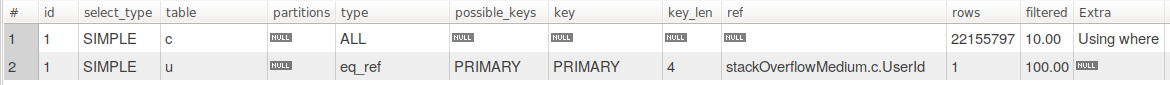
\includegraphics[scale =0.4]{explain7.png} 
	\caption{Przykład 1}
\end{figure}
\begin{spverbatim}
	SELECT p.Body from Posts p where p.Id = 875 union
	select c.`Text` from Comments c where c.PostID = 875;
\end{spverbatim}
\begin{figure}[H]
	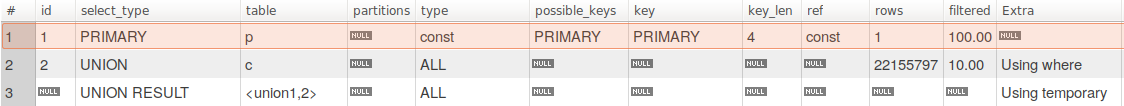
\includegraphics[scale =0.4]{explain8.png} 
	\caption{Przykład 2}
\end{figure}
\begin{spverbatim}
	SELECT * from Comments where UserId = (select id from Users where DisplayName = 'Jarrod Dixon');
\end{spverbatim}
\begin{figure}[H]
	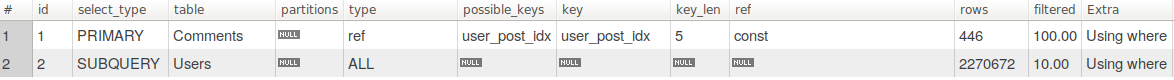
\includegraphics[scale =0.4]{explain9.png} 
	\caption{Przykład 3}
\end{figure}
\begin{spverbatim}
	SELECT * FROM Comments where UserID in ( select UserId from Posts group by UserId having count(*) > 10);
\end{spverbatim}
\begin{figure}[H]
	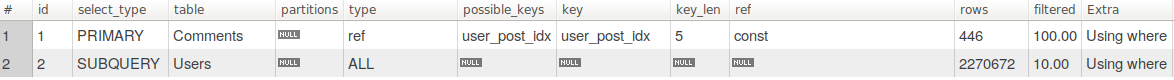
\includegraphics[scale =0.4]{explain9.png} 
	\caption{Przykład 4}
\end{figure}
\begin{spverbatim}
	SELECT * FROM Comments where UserID in ( select UserId from Posts group by UserId having count(*) > 10);
\end{spverbatim}
\begin{figure}[H]
	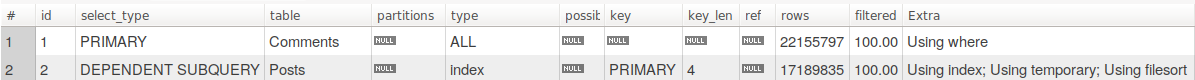
\includegraphics[scale =0.4]{explain10.png} 
	\caption{Przykład 5}
\end{figure}
\begin{spverbatim}
	SELECT * FROM Posts  WHERE OwnerUserId in (select id from Users where Reputation>1000 UNION SELECT UserId FROM Comments WHERE Score >10)
\end{spverbatim}
\begin{figure}[H]
	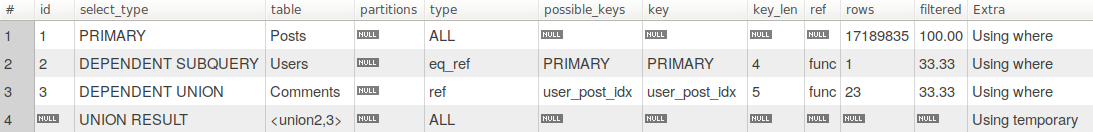
\includegraphics[scale =0.4]{explain11.png} 
	\caption{Przykład 6}
\end{figure}
\begin{spverbatim}
	SELECT * FROM Comments WHERE UserId = (select @var1 from Users where DisplayName = 'Jarrod Dixon');
\end{spverbatim}
\begin{figure}[H]
	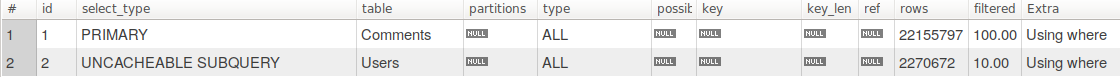
\includegraphics[scale =0.4]{explain12.png} 
	\caption{Przykład 7}
\end{figure}
\begin{spverbatim}
SELECT * FROM Comments limit 10;
\end{spverbatim}
\begin{figure}[H]
	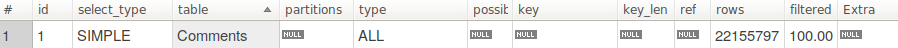
\includegraphics[scale =0.4]{explain13.png} 
	\caption{Przykład 8}
\end{figure}

\paragraph{Kolumna ID}\leavevmode\\
Kolumna id zawiera numer zapytania, którego dotyczy. W przypadku zapytań z podzapytaniami, podzapytania w dyrektywie FROM oraz zapytań z słowem kluczowym JOIN podzapytania numerowane są najczęściej względem ich występowania w zapytaniu. Kolumna ID może przyjąć również wartość NULL, w przypadku polecenia UNION (przykład 2).

\paragraph{Kolumna select\textunderscore type}\leavevmode\\
Kolumna select\textunderscore type pokazuje, czy rekord jest prostym, czy złożonym zapytaniem SELECT. 
Wartość \textbf{SIMPLE} oznacza, że zapytanie nie zawiera podzapytań, oraz nie używa klauzuli UNION.

Jeżeli natomiast zapytanie zawiera podzapytania lub wykorzystuje klauzulę UNION, to rekord dla kolumny select\textunderscore type przyjmie wartość \textbf{PRIMARY} (przykład 2). Jeżeli rekord dotyczy podzapytania oznaczonego jako PRIMARY, to będzie oznaczony jako \textbf{SUBQUERY} (przykład 3). Jako \textbf{UNION} zostaną oznaczone zapytania, które są drugim i kolejnym zapytaniem w klauzuli UNION. Pierwsze zapytanie zostanie oznaczone tak samo, jakby było wykonywane jako zwykłe zapytanie SELECT (przykład 2). \textbf{DERIVED} oznacza, że zapytanie jest umieszczone jako podzapytanie w klauzuli FROM, jest wykonywane rekurencyjnie i wyniki są umieszczane w tabeli tymczasowej. Wartość \textbf{UNION RESULT} oznacza wiersz, jako polecenie SELECT użyte do pobrania wyników z tabeli tymczasowej użytej przy poleceniu UNION (przykład 2). Jeśli polecenie SELECT zależy od danych znajdujących się w podzapytaniu lub znajdujących się w wyniki klazuli UNION, to zostanie oznaczone odpowiednio jako \textbf{DEPENDENT SUBQUERY} (przykład 5) lub \textbf{DEPENDENT UNION} (Przykład 6). Dodatkowo w przypadku, jeżeli wynik zwracany jest z \textit{zmaterializowanego widoku (eng. materialized view)}, zapytanie zostanie oznaczone jako \textbf{MATERIALIZED}. W przykładzie 7, który jest oczywiście nonsensowny, ale dobrze obrazuje sytuację, kiedy jako select\textunderscore type otrzymamy wartość \textbf{UNCACHABLE\textunderscore SUBQUERY}, która oznacza, że coś w podzapytaniu uniemożliwiło jego buforowanie. Analogiczną sytuację mamy, jeżeli wiersz zostanie oznaczony jako \textbf{UNCACHABLE\textunderscore UNION}, ale w tym przypadku niemożliwe jest oczywiście buforowanie wyników polecenia UNION.

\paragraph{Kolumna table}\leavevmode\\
Kolumna \textit{table} w większości przypadków zawiera nazwę tabeli lub jej alias, do której odnosi się dany wiersz wyniku polecenia \textit{EXPLAIN}. W przypadku gdy zapytanie dotyczy tabel tymczasowych możemy zobaczyć np. table: <union1,2> (przykład 2), co oznacza, że zapytanie dotyczy tabeli tymczasowej stworzonej na podstawie polecenia \textit{UNION} na tabelach z wierszy o id 1 oraz 2.
Odczytując kolejno wartości kolumny \textit{table} możemy dowiedzieć się, w jakiej kolejności optymalizator MySQL zdecydował się ułożyć zapytania. 

\paragraph{Kolumna Type}\leavevmode\\
Kolumna \textit{Type} informuje o tym, w jaki sposób MySQL będzie przetwarzał wiersze w tabeli. Poniżej przedstawiono najważniejsze metody dostępu do danych, w kolejności od najgorszej do najlepszej.

\subparagraph{ALL}\leavevmode\\
Wartość \textit{ALL} informuje o tym, że serwer musi przeskanować całą tabelę w celu odnalezienia rekordów. Istnieją jednak wyjątki takie, jak w przykładzie 8, w którym polecenie \textit{EXPLAIN} pokazuje, że będzie wykonywany pełny skan tabeli, a w rzeczywistości dzięki użyciu polecenia \textit{LIMIT} zapytanie będzie wymagało jedynie 10 rekordów.

\subparagraph{index}\leavevmode\\
MySQL skanuje wszystkie wiersze w tabeli, ale może wykonać to w porządku w jakim jest przechowywane w indeksie, dzięki czemu unika sortowania. Największą wadą jest konieczność odczytu całej tabeli w kolejności indeksu, co zazwyczaj oznacza pobieranie danych z dysku w losowej kolejności. Jeżeli w kolumnie \textit{extra} jest dodatkowo zawarta informacja "Using Index" oznacza to, że MySQL wykorzystuje idenks pokrywający (opisany w dalszej części pracy) i nie wymaga odczytywania indeksów z dysku.

\subparagraph{range}\leavevmode\\
Wartość \textit{range} oznacza ograniczone skanowanie zakresu. Takie skanowanie rozpoczyna się od pewnego miejsca indeksu, dzięki czemu nie musimy przechodzić przez cały indeks. Skanowanie indeksu powodują zapytania zawierające klauzulę \textit{BETWEEN} lub \textit{WHERE} z < lub >. Wady są takie same jak przy rodzaju \textit{index}

\subparagraph{index\textunderscore subquery}\leavevmode\\
TODO przyklad
\subparagraph{unique\textunderscore subquery}\leavevmode\\
TODO przyklad
\subparagraph{index merge}\leavevmode\\
TODO przyklad
\subparagraph{fulltext}\leavevmode\\
TODO przyklad

\subparagraph{ref}\leavevmode\\
Jest to wyszukiwanie, w którym MySQL musi przeszukać jedynie indeks w celu znalezienia rekordu opowiadającego pojedyńczej wartości.
Przykładem takiego zapytania może być wyszukiwanie numerów postów danego użytkownika w tabeli \textit{Comments} zawierającej indeks typu \textit{BTREE} na kolumnach \textit{UserId} oraz \textit{PostId}.

\begin{spverbatim}
	SELECT PostId FROM Comments WHERE UserId = 10;
\end{spverbatim}
Dodatkowo odmianą dostępu \textit{ref} jest dostępd \textit{ref\textunderscore or\textunderscore null}, który oznacza, że wymagany jest dodatkowy dostęp w celu sprawdzenia wartości NULL.


\subparagraph{eq\textunderscore ref}\leavevmode\\

Jest to najlepsza możliwa forma złączenia. Oznacza, że każdy wiersz z pierwszej tabeli jest dopasowywany do pierwszego zwróconego wyniku w drugiej tabeli i nie jest wymagane dalsze przeszukiwanie. Z tego rodzaju złączeniem mamy do czynienia, jeżeli wszystkie kolumny używane do złączenia są kluczem głównym lub indeksem "NOT NULL UNIQUE". Przykładem takiego zapytania jest złączenie wszystkich komentarzy z postami bazując na kluczu głównym Id z tabeli Posts. 

\begin{spverbatim}
	SELECT * FROM Comments c JOIN Posts p ON c.PostId = p.id;
\end{spverbatim}

\subparagraph{const}\leavevmode\\
Przeważnie występuje w przypadku użycia w klauzuli WHERE wartości z indeksu głównego. Wtedy MySQL musi znaleźć tylko jedną wartość, która jest kluczem. Dla przykładu w bazie StackOverflow może to być zapytanie pobierające komentarz bazując na Id.
\begin{spverbatim}
	EXPLAIN SELECT * FROM Comments WHERE id = 93;
\end{spverbatim}

\subparagraph{NULL}\leavevmode\\
Oznacza, że serwer nie wymaga dostepu do tabeli czy indeksu i może zwrócić wartość już podczas fazy optymalizacji. Przykładem takiego zapytania może być zwrócenie minimalnej wartości z indeksu tabeli.

\begin{spverbatim}
	SELECT MIN(UserId) FROM Comments;
	#Tabela Comments zawiera indeks BTREE na kolumnie UserID
\end{spverbatim}

\paragraph{Kolumna Possible\textunderscore keys}\leavevmode\\

Komulna possible\textunderscore keys zawiera listę indeksów, które optymalizator brał pod uwagę podczas tworzenia planu wykonania zapytania. Lista tworzona jest na początku procesu optymalizacji zapytania.

\paragraph{Kolumna key}\leavevmode\\

Kolumna \textit{key} sygnalizuje, który indeks został wybrany do optymalizacji dostępu do tabeli.

\paragraph{Kolumna key\textunderscore len}\leavevmode\\
Wartość oznacza jaki jest rozmiar bajtów użytego indeksu. W przypadku, kiedy zostanie wykorzystana jedynie część kolumn indeksu, wtedy wartość \textit{key\textunderscore len} będzie odpowiednio mniejsza. Istotny jest fakt, że rozmiar jest zawsze maksymalnym rozmiarem zindeksowanych kolumn, a nie rzeczywistą liczbą bajtów danych używanych przez tabelę.

\paragraph{Kolumna ref}\leavevmode\\
Kolumna pokazuje, które kolumny z innych tabel lub zmienne z innych tabel zostaną wykorzystane do wyszukania wartości w indeksie podanym w kolumnie \textit{key}. W przykładzie 1, widzimy, że do przeszukania indeksu tabeli Posts została wykorzystana kolumna UserId z tabeli Comments (alias c). Wartość \textit{const} oznacza, że do przeszukania wartości została wykorzystana stała podana np. w klauzuli WHERE (Przykład 2).

\paragraph{Kolumna rows}\leavevmode\\
Kolumna wskazuje oszacowaną liczbę wierszy, które MySQL będzie musiał odczytać w celu znalezienia szukanych rekordów. Istotne jest to, że jest to liczba przeszukiwanych rekordów na danym poziomie zagnieżdenia pętli planu złączenia. To znaczy, że nie jest to całkowita liczba rekordów, a jedynie liczba rekordów w jednej pętli złączenia danej tabeli. W przypadku złączenia sumaryczna liczba przeszukiwanych nie jest sumą wartości z wszystkich wierszy, a iloczynem wartości z wierszy biorących udział w złączeniu. W przykładzie 9, łączna suma wierszy, które muszą zostać przeszukane nie wynosi 1574
\begin{spverbatim}
	SELECT * FROM Posts p JOIN PostTypes pt ON p.PostTypeId = pt.Id;
\end{spverbatim}
\begin{figure}[H]
	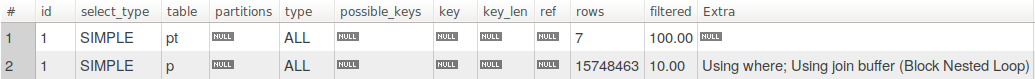
\includegraphics[scale =0.4]{explain14.png} 
	\caption{Przykład 9}
\end{figure}
Dodatkowo należy wziąć pod uwagę, że są to jedynie szacunkowe wartości, które w praktyce mogą być zupełnie nie prawidłowe. Ponadto optymalizator podczas szacowania wartości w kolumnie \textit{rows} nie bierze pod uwagę klauzli \textit{LIMIT}.

\paragraph{Kolumna filtered}\leavevmode\\
Kolumna \textit{filtered} pojawia się jedynie podczas użycia polecenia \textit{EXPLAIN EXTENDED}. Wskazuje na wartość oszacowaną przez optymalizator, która informuje ile rekordów może zostać odfiltrowane za pomocą klauzuli WHERE. W przykładzie 4 optymalizator MySQL oszacował, że jedynie 10 procent użytkowników napisało w sumie więcej niż 10 komentarzy. 

\paragraph{Kolumna extra}\leavevmode\\
Kolumna \textit{extra} zawiera informacje, których nie udało się zamieścić w pozostałych kolumnach. Poniżej przedstawione zostanie kilka najważniejszych informacji, które mogą znaleźć się w tej kolumnie.

\begin{itemize}
	\item 'Using index' - MySQL użyje indeksu pokrywającego zamiast dostępu do tabeli.
	\item 'Using where' - oznacza, że MySQL przeprowadzi filtrowanie danych już po wyciągnięciu danych z tabeli. Często jest to informacja, którą warto przemyśleć pod kątem stworzenia nowego (lub modyfikacji istniejących) indeksów.
	\item 'Using temporary' - do sortowania wyników używana jest tabela tymczasowa.
	\item 'Using filesort' - sortowanie nie może wykorzystywać indeksu, więc wiersze są sortowane za pomocą jednego z algorytmów sortowania.
	
\end{itemize}